\documentclass[11pt]{article}
\usepackage{icmlko}
\begin{document}

\title{음수 전이가 사라졌다 --- 원핫을 떼서가 아니라 일반화되는 이름표를 하나 더 줘서}
\author{월드모델 실험실}
\date{노트 417 · 2026년 8월 2일}
\maketitle

\begin{abstract}
노트 372부터 407까지, 이 실험실이 목표로 삼은 자리는 하나였다 --- \emph{안 본
도메인에서 판이 거꾸로 줄을 선다.} KR 만화가 $-0.1261$(노트 398), 범인은
도메인 원핫(노트 399), 드롭아웃으로는 못 피한다(노트 400), 깊이가 값을 반으로
깎는다(노트 407). 그동안 처방은 언제나 \textbf{원핫을 떼는 것}이었고 값은
언제나 판이었다.

노트 413에서 \texttt{grp} --- 집단 표지 축, 기획 시점 정보, 일곱 도메인 ---
를 채택했다. 그때 사전 등록이 \textbf{거꾸로} 틀렸다: grp 가 \emph{안 덮는}
도메인이 덮는 도메인의 4.7배를 벌었다. 읽기는 이랬다 --- grp 가 도메인 사이
분산을 흡수하니 공유 축이 도메인 \emph{안}에서 일하고, \textbf{공유 축에
제일 많이 기대던 도메인이 제일 크게 번다.}

\textbf{그 논리의 끝은 학습에 아예 없는 도메인이다.} grp 를 넣고 전이를
다시 쟀다.

\begin{center}
\begin{tabular}{lrr}
\hline
 & KR 만화 (\textbf{안 본 도메인}) & JP 만화 (학습에 듦) \\
\hline
깊이4 · grp 없음 (노트 399) & $-0.1261$ & $+0.3196$ \\
깊이6 · grp 없음 (노트 407) & $-0.0822$ & $+0.3277$ \\
\textbf{깊이6 · grp 있음} & $\mathbf{+0.2128}$ & $+0.3286$ \\
\hline
\end{tabular}
\end{center}

\textbf{음수 전이가 없어졌다.} 그것도 원핫을 \emph{그대로 둔 채}다. JP 는
$+0.3277 \to +0.3286$ 으로 안 움직이니 전체가 밀린 것이 아니다. 안 본
도메인이 학습 도메인의 \textbf{65\%} 까지 온다 --- 직전까지 음수였다.
\end{abstract}

\section{그리고 부호가 뒤집혔다}

grp 든 판에서 원핫을 떼면 KR 이 \textbf{내려간다}: $+0.2128 \to +0.1563$.
노트 399·407 에서는 떼는 쪽이 나았다($-0.1261 \to +0.0797$). \textbf{같은
조작의 부호가 반대다.}

판 쪽도 같이 봤다. grp 든 판에서 원핫 제거의 판 손해는
$\mathbf{+0.0004 \cdot 6/12}$ --- 두 팔이 \textbf{구별되지 않는다}
(깊이4 $-0.0117$ → 깊이6 $-0.0052$ → 지금 0). 노트 399가 적은 긴장
(\emph{판은 지키라 하고 목표는 빼라 한다})에서 \textbf{판이 침묵한 첫
순간}인데, 바로 그때 \textbf{목표 쪽도 남기라고 한다.}

사전 등록한 채택 기준 --- ① KR 없음이 양수 ② 있음보다 큼 ③ JP 안 내림
--- 중 ②가 걸렸다. \textbf{원핫을 유지한다.} 이번엔 두 축이 처음으로
같은 말을 한다.

\section{왜 grp 가 전이를 사나}

원핫은 안 본 도메인에서 \textbf{전부 0} 인 좌표를 준다 --- 학습에 한 번도
안 나온 자리다(노트 399). grp 는 다르다. \textbf{국가 · 포맷 · 매체 ·
연령등급 · 무료 여부}는 새 작품에도 있다. 도메인 이름표가 아니라
\textbf{도메인을 가로지르는 성질}이라서, 안 본 도메인도 그 열에서는
낯선 자리에 안 선다.

그림 (다)가 노트 413의 기울기를 끝까지 그린 것이다 --- grp 로 얻는 값이
\textbf{덮인 일곱 $+0.0045$ · 안 덮인 넷 $+0.0212$ · 학습에 아예 없는 KR
$+0.2950$} 로 커진다. \textbf{공유 축에 기댈수록 많이 번다}는 한 문장이
세 눈금 다 설명한다.

\section{노트 413의 수치를 바로잡는다}

노트 413이 grp 덮음을 \textbf{여덟 도메인}이라 적고 덮인 평균 $+0.0042$ ·
안 덮인 $+0.0278$(6.7배)이라 했다. 틀렸다 --- grp 는 \textbf{일곱}을 덮고
\textbf{만화는 안 덮는다}(모듈이 만화를 안 낸다). 대본이 덮음 집합을 손으로
적으면서 만화를 덮인 쪽에 넣었다. 바로잡으면 \textbf{덮인 일곱 $+0.0045$ ·
안 덮인 넷 $+0.0212$, 4.7배}다. 방향과 채택은 그대로다.

\section{남은 것}

\begin{tabular}{lp{7.2cm}}
\hline
전이 점이 아직 둘 & KR 만화 · 비게임 앱. \textbf{$+0.2128$ 의 오차를
모른다} --- 다음 사이클의 첫 일 \\
비게임 앱 & 노트 398에서 $+0.08$ 이었다. grp 로 다시 재야 한다 \\
일반화되는 이름표 더 & grp 가 이만큼 했다면 같은 꼴(도메인을 가로지르는
기획 시점 범주)이 더 있나 \\
\hline
\end{tabular}

\begin{figure}[h]
\centering
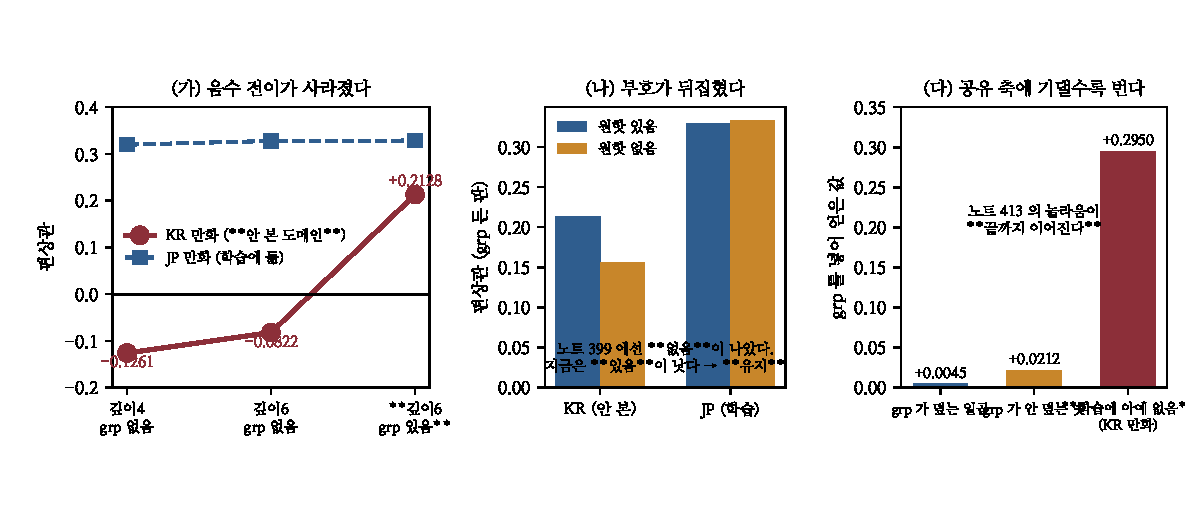
\includegraphics[width=\textwidth]{figs/fig417.pdf}
\caption{(가) 안 본 도메인의 편상관이 $-0.1261 \to +0.2128$ 로 올라온다.
JP 는 안 움직인다. (나) grp 든 판에서는 원핫을 떼면 오히려 KR 이 내린다.
(다) grp 의 이득은 공유 축에 기댈수록 크다 --- 끝은 학습에 아예 없는
도메인이다.}
\end{figure}

\end{document}
